\section{Auswertung}
\label{sec:Auswertung}
Sämtliche im Folgenden durchgeführten Ausgleichsrechnungen werden mit der \emph{curve fit} Funktion aus dem für \emph{Python} geschriebenen package \emph{NumPy}\cite{scipy} durchgeführt. Fehlerrechnungen werden mit dem für \emph{Python} geschriebenen package \emph{Uncertainties}\cite{uncertainties} ausgeführt.

\subsection{Messdaten der ersten Heizrate}
\label{sec:hohe_heizrate}
Bei der ersten Durchführung ist eine Heizrate von \SI{2}{\kelvin\per\minute} angestrebt worden. Die dazugehörigen Messdaten sind in Abbildung \ref{fig:Auswertung_1_2} dargestellt.


\begin{figure}
\centering
\begin{subfigure}{.5\textwidth}
	\centering
	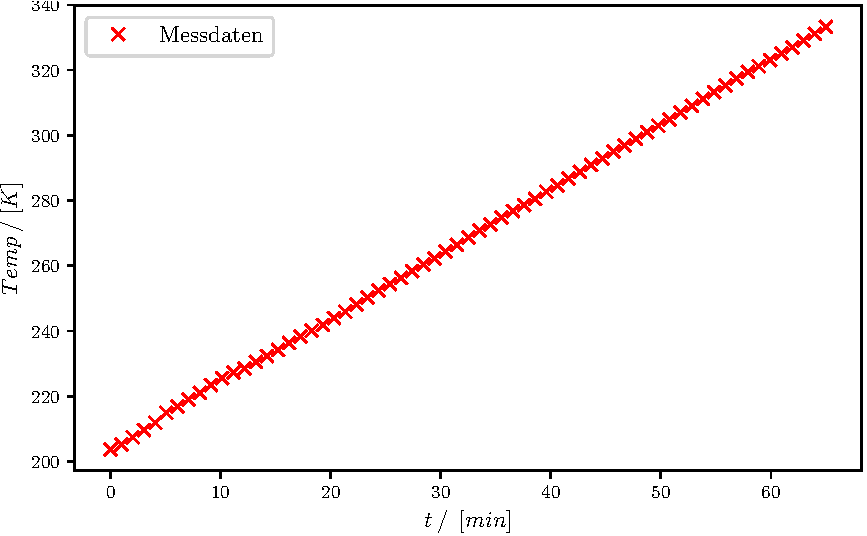
\includegraphics[width=1\textwidth]{build/1_Temp_Time.pdf}
	\caption{}
	\label{fig:Auswertung_1}
\end{subfigure}%
\begin{subfigure}{.5\textwidth}
	\centering
	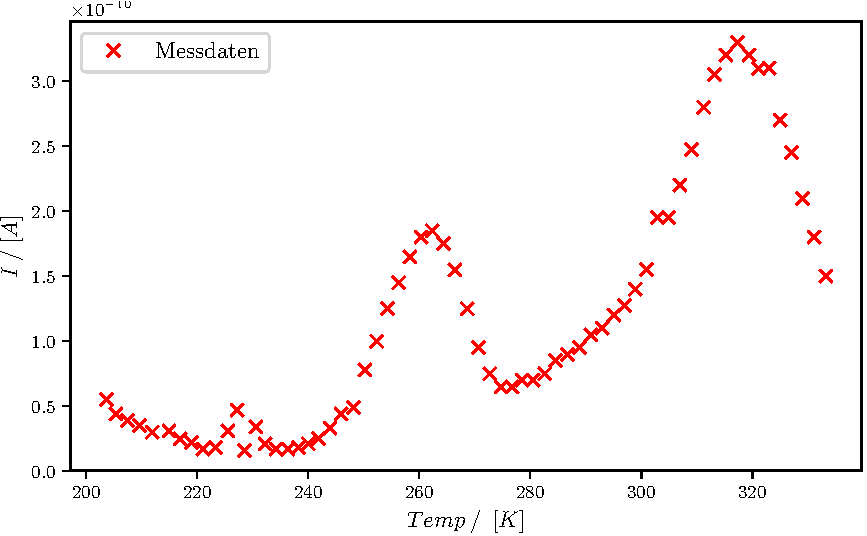
\includegraphics[width=1\textwidth]{build/1_Temp_current.pdf}
	\caption{}
	\label{fig:Auswertung_2}
\end{subfigure}
\caption{Temperaturgradient während der Messung und aufgenommene Messdaten.}
\label{fig:Auswertung_1_2}
\end{figure}

Zur Berücksichtigung des Untergrunds wird die Funktion 
\begin{align}
	I(T)=a\cdot\exp{(bT)}+c \;,
	\label{fkt:fit1}
\end{align}
verwendet. Die in Abbildung \ref{fig:Auswertung_3} gelb markierten Messwerte werden als Untergrund interpretiert und dienen der Fitfunktion als Datengrundlage. Die Messdaten als auch der Untergrundfit sind in Abbildung \ref{fig:Auswertung_4} dargestellt.


\begin{figure}
\centering
\begin{subfigure}{.5\textwidth}
	\centering
	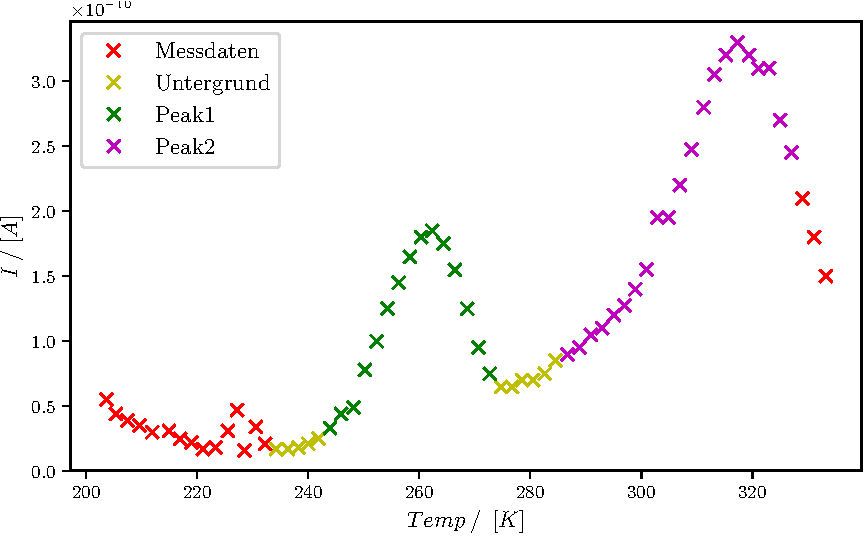
\includegraphics[width=1\textwidth]{build/1_Temp_current_background_peak_withoutfit.pdf}
	\caption{}
	\label{fig:Auswertung_3}
\end{subfigure}%
\begin{subfigure}{.5\textwidth}
	\centering
	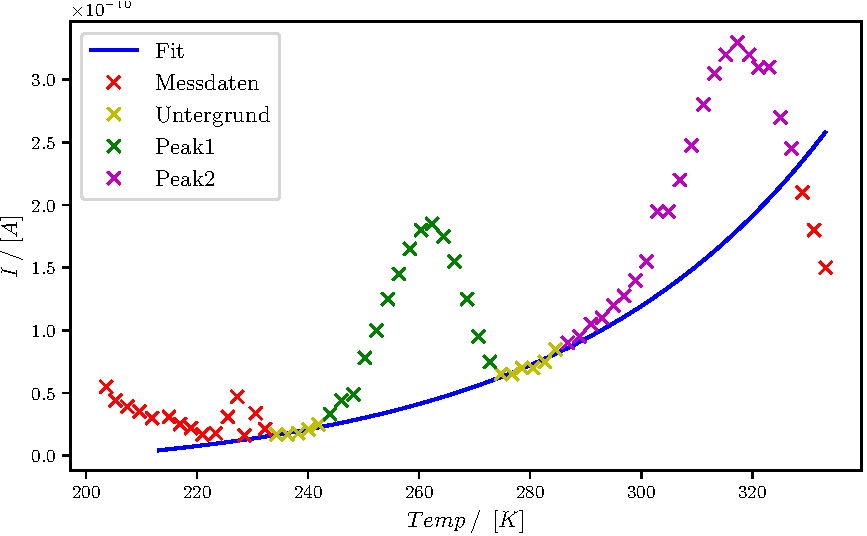
\includegraphics[width=1\textwidth]{build/1_Temp_current_background_peak.pdf}
	\caption{}
	\label{fig:Auswertung_4}
\end{subfigure}
\caption{Darstellung der als Untergrund definierten Messwerte und der daraus resultierenden Ausgleichsrechnung.}
\label{fig:Auswertung_3_4}
\end{figure}

Die Ausgleichsrechnung liefert folgende Parameter:
\begin{align}
  a &= \SI{0.24+-0.62}{\pico\ampere}
 \\
  b &= \SI{0.0211+-0.0082}{\per\kelvin}
 \\
  c &= \SI{-0.02+-0.13}{\nano\ampere}

\end{align}

In Abbildung \ref{fig:Auswertung_5_6} sind die Messdaten der beiden Maxima unter Berücksichtigung des Untergrunds nach \ref{fkt:fit1} aufgetragen.


\begin{figure}
\centering
\begin{subfigure}{.5\textwidth}
	\centering
	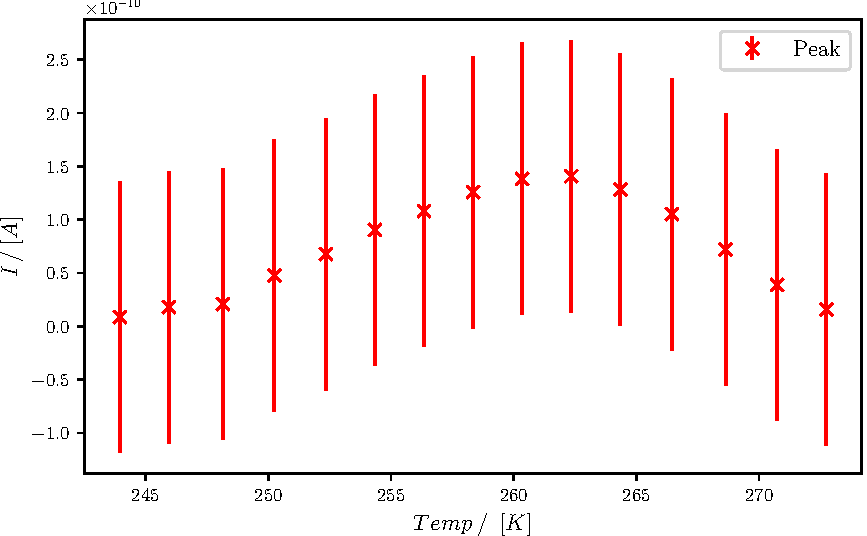
\includegraphics[width=1\textwidth]{build/1_Temp_current_peak.pdf}
	\caption{}
	\label{fig:Auswertung_5}
\end{subfigure}%
\begin{subfigure}{.5\textwidth}
	\centering
	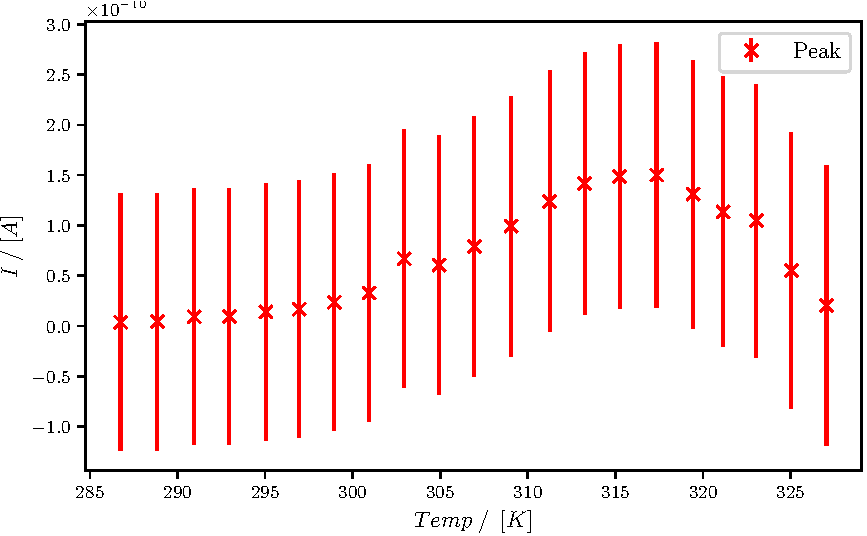
\includegraphics[width=1\textwidth]{build/1_Temp_current_peak2.pdf}
	\caption{}
	\label{fig:Auswertung_6}
\end{subfigure}
\caption{separate Darstellung der beiden Maxima, korrigiert um den Untergrund.}
\label{fig:Auswertung_5_6}
\end{figure}

\subsubsection{Bestimmung von $W$ mit der "Flanken"-Methode}

Die ersten 10 Messwerte des erstens Maximums und die ersten 15 Messwerte des zweiten Maximums werden der positiven Flanke zugeordnet. Mit diesen Teilintervallen wird anschießend die Ausgleichsrechnung nach Gleichung \eqref{Formel5} durchgeführt. Die logarithmierten Ströme und die jeweilige Ausgleichsrechnung sind in Abbildung \ref{fig:Auswertung_7_8} zusehen.


\begin{figure}
\centering
\begin{subfigure}{.5\textwidth}
	\centering
	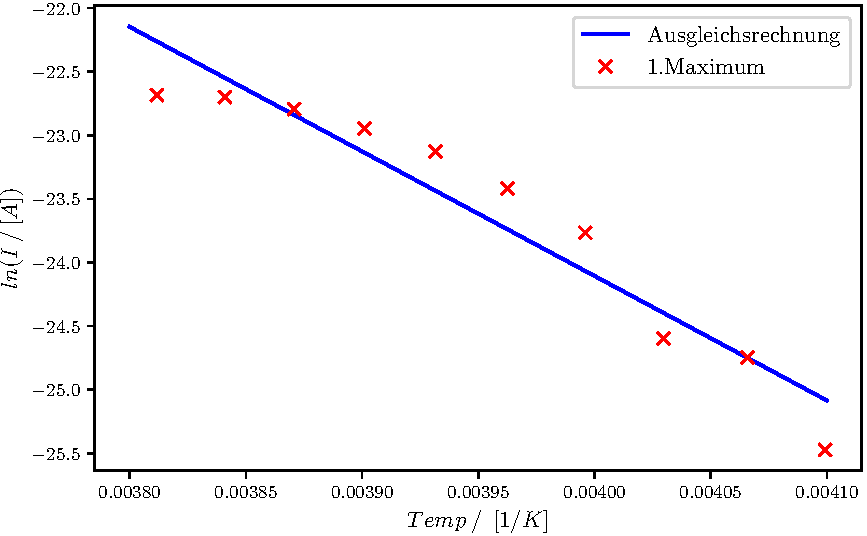
\includegraphics[width=1\textwidth]{build/1_Temp_current_peak_log_fit.pdf}
	\caption{}
	\label{fig:Auswertung_7}
\end{subfigure}%
\begin{subfigure}{.5\textwidth}
	\centering
	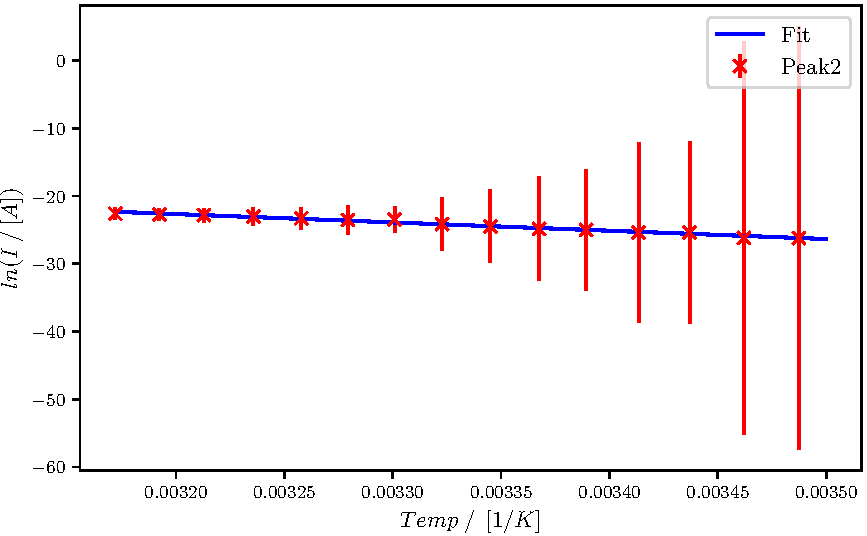
\includegraphics[width=1\textwidth]{build/1_Temp_current_peak2_log_fit.pdf}
	\caption{}
	\label{fig:Auswertung_8}
\end{subfigure}
\caption{einfach logarithmierte Darstellung der Maxima mit Ausgleichsrechnung.}
\label{fig:Auswertung_7_8}
\end{figure}

Aus den Fitparametern ergibt sich die Aktivierungsenergien $W$ zu

\begin{align}
	W_{Peak1} = \SI{0.844+-0.089}{\electronvolt}
  \quad \text{und} \quad W_{Peak2} = \SI{1.059+-0.045}{\electronvolt}
\;.
\end{align}

Für die Berechnung der minimalen Relaxationszeit $\tau_0$ nach Gleichung \eqref{Formel8} wird die jeweilige Heizrate $b$ benötigt.
Diese wird für jedes Maximum individuell berechnet, indem die gemessenen Temperatur im Maximum gegen die Zeit aufgetragen wird, um eine lineare Ausgleichsrechnung durchzuführen. Die in Abbildung \ref{fig:Auswertung_11_12} dargestellt Vorgehensweise ergibt eine Heizrate von 

\begin{align}
	b_{Peak1} = \SI{1.912+-0.005}{\kelvin\per\minute}
  \quad \text{und} \quad b_{Peak2} = \SI{1.922+-0.005}{\kelvin\per\minute}
\;.
\end{align}

\begin{figure}
\centering
\begin{subfigure}{.5\textwidth}
	\centering
	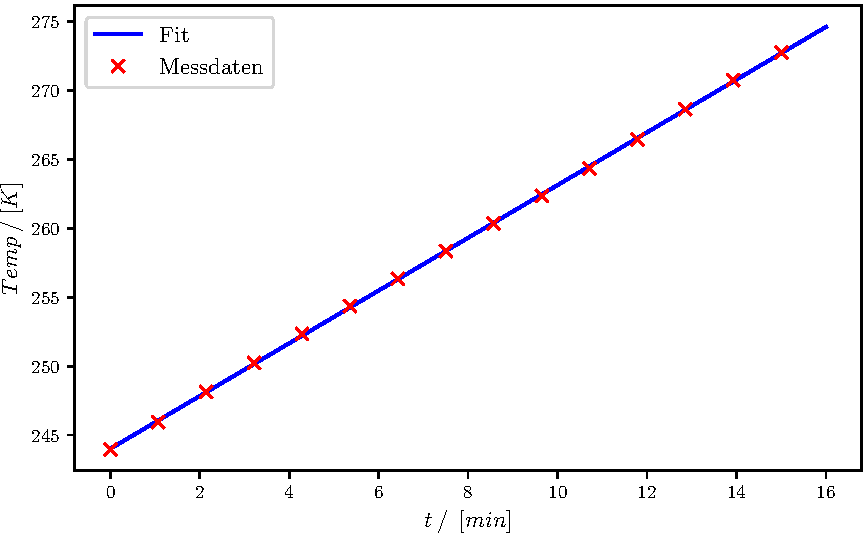
\includegraphics[width=1\textwidth]{build/1_Temp_Time_Peak1.pdf}
	\caption{}
	\label{fig:Auswertung_11}
\end{subfigure}%
\begin{subfigure}{.5\textwidth}
	\centering
	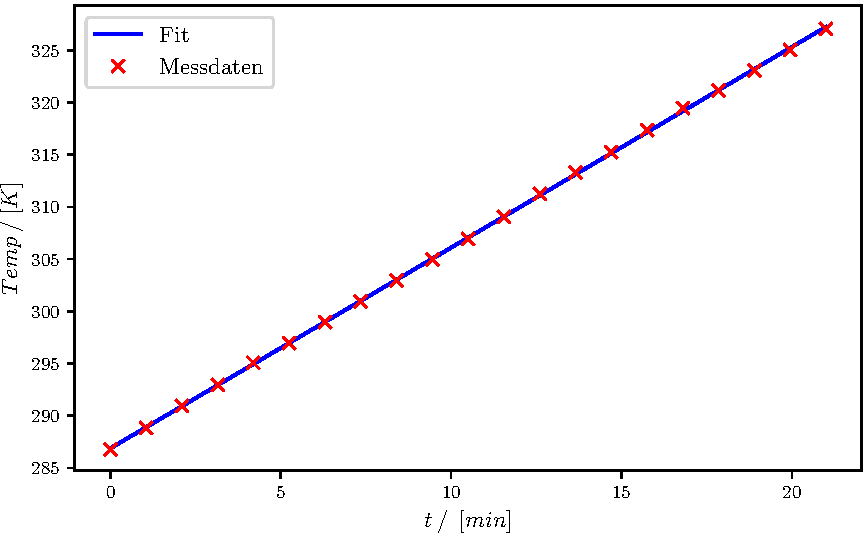
\includegraphics[width=1\textwidth]{build/1_Temp_Time_Peak2.pdf}
	\caption{}
	\label{fig:Auswertung_12}
\end{subfigure}
\caption{Darstellung der Temperatur gegen die Zeit zur Ermittlung der Heizrate während der Durchführung.}
\label{fig:Auswertung_11_12}
\end{figure}

Daraus berechnen sich mit

\begin{align}
	T_{max,Peak1} = \SI{264.35}{\kelvin}
  \quad \text{und} \quad T_{max,Peak2} = \SI{317.35}{\kelvin}
\;.
\end{align}

die Relaxationszeiten zu

\begin{align}
	\tau_{0,Peak1} = \SI{0.3+-1.2}{\pico\second}
  \quad \text{und} \quad \tau_{0,Peak2} = \SI{0.06+-0.11}{\pico\second}
\;.
\end{align}



\subsubsection{Bestimmung von $W$ mit der "Vollpeak"-Methode}

Bei diesem Verfahren werden alle Messwerte der Maxima verwendet, wie in Abbildung \ref{fig:Auswertung_5_6} dargestellt. Für die Ausgleichsrechnung ist es erforderlich das Integral in der Gleichung

\begin{align}
	\ln(\int_{T}^{T_{\infty}} I(T’) dT’) - \ln(I(T))=\ln(\tau_0\cdot b) + \frac{W}{k_B T}
	\label{eq:auswertung_integral}
\end{align}

zu bestimmen. Dabei stehen die Grenzen $T$ bzw. $T_{\infty}$ für den letzten bzw. des ersten Wert des Maximums. Zur nummerischen Berechnung wird die Sehnentrapezformel verwendet. In Abbildung \ref{fig:Auswertung_9_10} sind die Messwerte und die Ausgleichsreichung dargestellt, wobei der linke Ausdruck der Fitfunktion durch ein $\Omega$ abgekürzt wird.


\begin{figure}
\centering
\begin{subfigure}{0.5\textwidth}
	\centering
	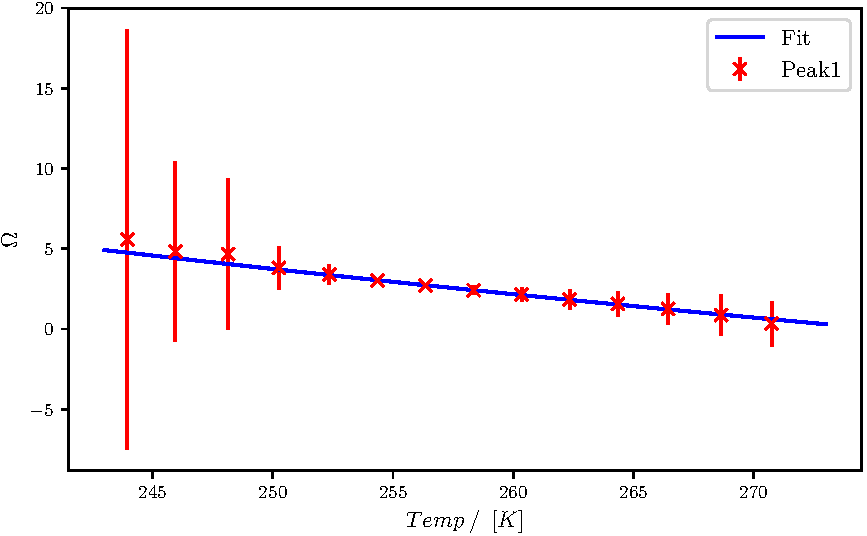
\includegraphics[width=1\textwidth]{build/1_Temp_current_peak_log_3.pdf}
	\caption{}
	\label{fig:Auswertung_9}
\end{subfigure}%
\begin{subfigure}{0.5\textwidth}
	\centering
	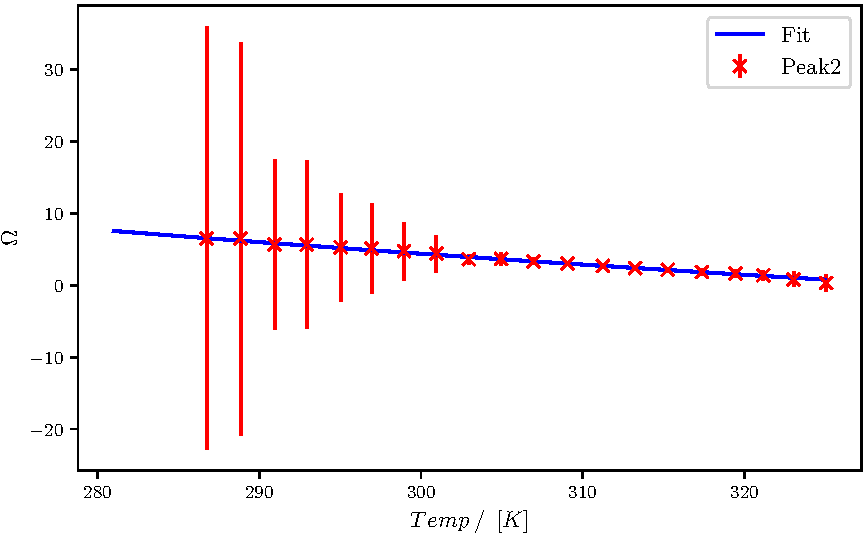
\includegraphics[width=1\textwidth]{build/1_Temp_current_peak2_log_3.pdf}
	\caption{}
	\label{fig:Auswertung_10}
\end{subfigure}
\caption{Darstellung der Messwerte mit Ausgleichsrechnung nach \ref{eq:auswertung_integral}.}
\label{fig:Auswertung_9_10}
\end{figure}

Aus den Fitparametern ergeben sich die Aktivierungsenergien 
\begin{align}
	W_{Peak1} = \SI{0.881+-0.017}{\electronvolt}
  \quad \text{und} \quad W_{Peak2} = \SI{1.211+-0.035}{\electronvolt}
\;.
\end{align}

Durch exponentieren des Fitparamters, der die Relation $\ln(\tau_0\cdot b)$ darstellt und anschließendem dividieren durch die zuvor berechnete Heizrate $b$, berechnet sich die minimale Relaxationszeit zu

\begin{align}
	\tau_{0,Peak1} = \SI{38+-30}{\atto\second}
  \quad \text{und} \quad \tau_{0,Peak2} = \SI{0.19+-0.25}{\atto\second}
\;.
\end{align}


\subsection{Messdaten der zweiten Heizrate}
Bei der zweiten Durchführung des Versuchs wurde eine Heizrate von \SI{1.5}{\kelvin\per\minute} angestrebt. Ansonsten erfolgt die Auswertung analog zu Kapitel \ref{sec:hohe_heizrate}.
In Abbildung \ref{fig:Auswertung_13_14} ist der Temperaturgradient während des Messvorgangs und der dazugehörige Strom dargestellt. 

\begin{figure}
\centering
\begin{subfigure}{.5\textwidth}
	\centering
	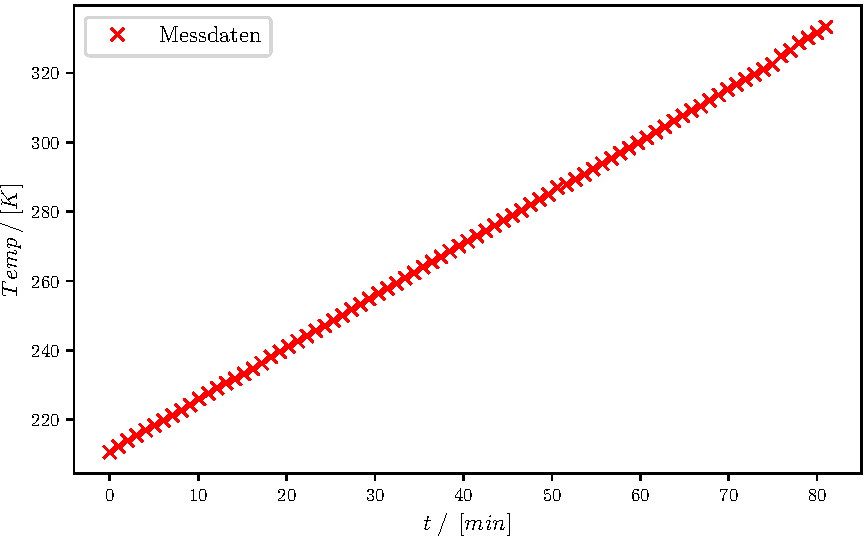
\includegraphics[width=1\textwidth]{build/2_Temp_Time.pdf}
	\caption{}
	\label{fig:Auswertung_13}
\end{subfigure}%
\begin{subfigure}{.5\textwidth}
	\centering
	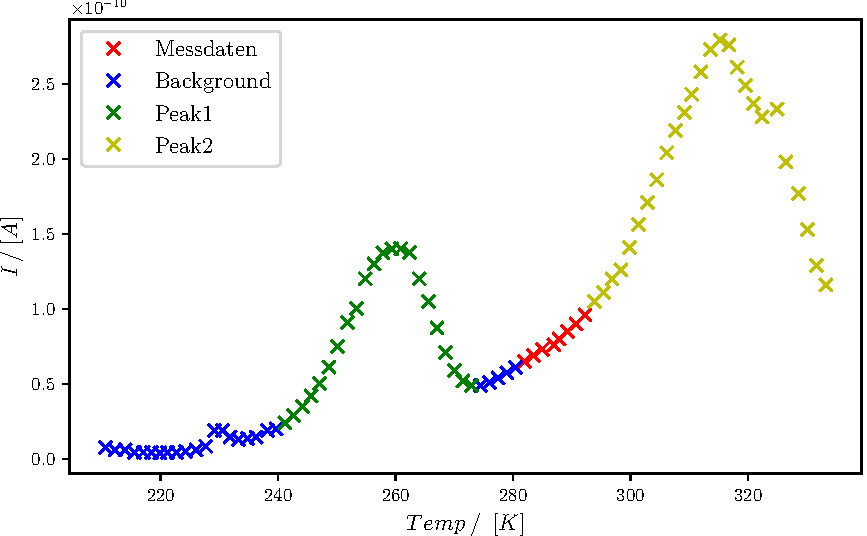
\includegraphics[width=1\textwidth]{build/2_Temp_current.pdf}
	\caption{}
	\label{fig:Auswertung_14}
\end{subfigure}
\caption{Temperaturgradient während der Messung und aufgenommene Messdaten.}
\label{fig:Auswertung_13_14}
\end{figure}

Erneut werden die Messdaten sowohl vor dem ersten Maximum als auch kurz danach als Untergrund angesehen. Dieses Teilintervall der Messdaten dient als Datengrundlage für die verwendete Fitfunktion (siehe Gleichung \ref{fkt:fit1}). In Abbildung \ref{fig:Auswertung_15} sind gruppierten Messdaten als auch der durchgeführte Untergrundfit darstellt. Die sich aus der Ausgleichsrechnung ergeben Parameter lauten:

\begin{align}
  a &= \SI{0.24+-0.62}{\pico\ampere}
 \\
  b &= \SI{0.0211+-0.0082}{\per\kelvin}
 \\
  c &= \SI{-0.02+-0.13}{\nano\ampere}

\end{align}

\begin{figure}
  \centering
  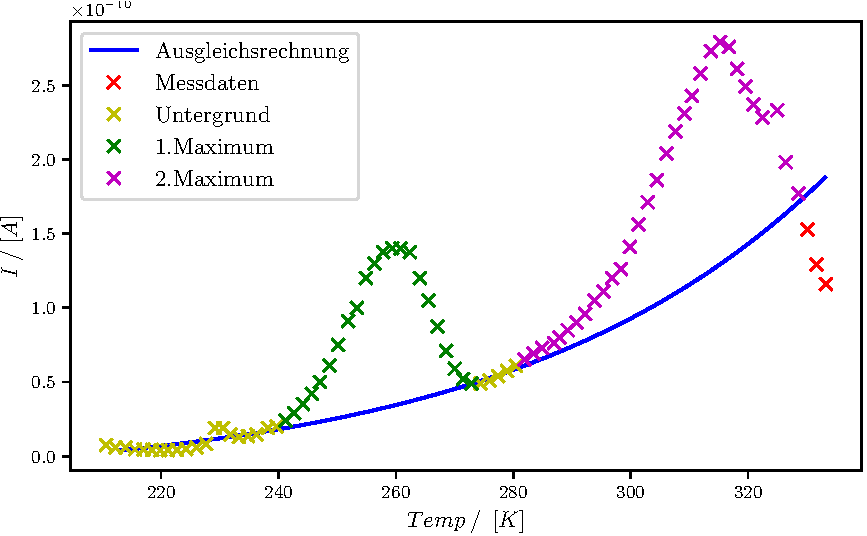
\includegraphics{build/2_Temp_current_background_peak.pdf}
  \caption{Darstellung der als Untergrund definierten Messwerte und der daraus resultierenden Ausgleichsrechnung.}
  \label{fig:Auswertung_15}
\end{figure}

Die Messdaten der beiden Maxima werden mit Hilfe der Ausgleichsrechnung korrigiert und anschließend separat in Abbildung \ref{fig:Auswertung_16_17} dargestellt.


\begin{figure}
\centering
\begin{subfigure}{.5\textwidth}
	\centering
	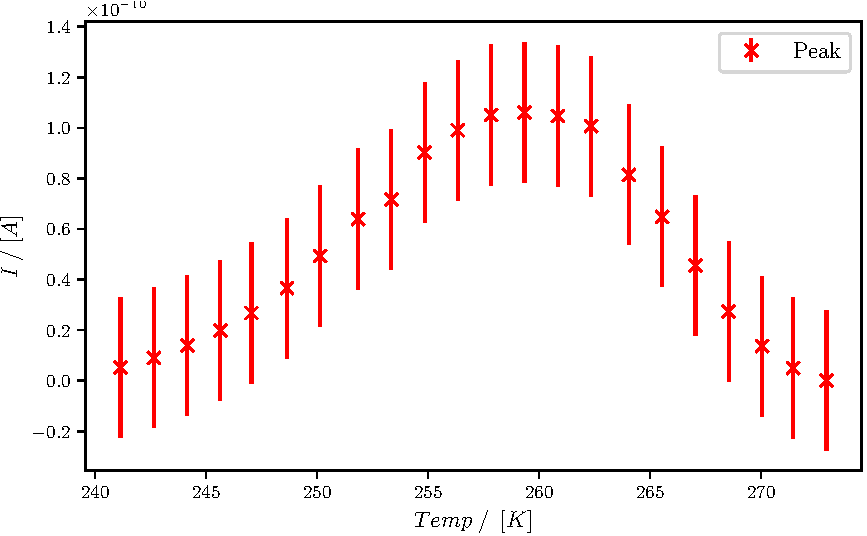
\includegraphics[width=1\textwidth]{build/2_Temp_current_peak.pdf}
	\caption{}
	\label{fig:Auswertung_16}
\end{subfigure}%
\begin{subfigure}{.5\textwidth}
	\centering
	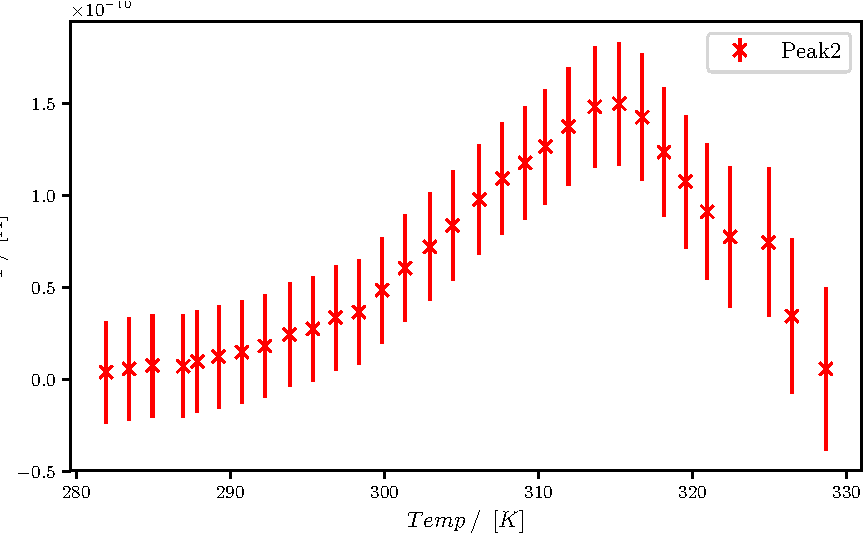
\includegraphics[width=1\textwidth]{build/2_Temp_current_peak2.pdf}
	\caption{}
	\label{fig:Auswertung_17}
\end{subfigure}
\caption{separate Darstellung der beiden Maxima, korrigiert um den Untergrund.}
\label{fig:Auswertung_16_17}
\end{figure}

\subsubsection{Bestimmung von $W$ mit der "Flanken"-Methode}

Die ersten 12 bzw 22 Messwerte des ersten bzw. zweiten Maximums werden als Werte der positiv ansteigenden Flanke interpretiert. Anschließend werden mit den Teilintervallen der Maxima, unter Verwendung von Gleichung \eqref{Formel5}, die Ausgleichsrechnungen durchgeführt. Das zuvor beschriebene Vorgehen in Abbildung \ref{fig:Auswertung_18_19} für beide Maxima separat dargestellt.

\begin{figure}
\centering
\begin{subfigure}{.5\textwidth}
	\centering
	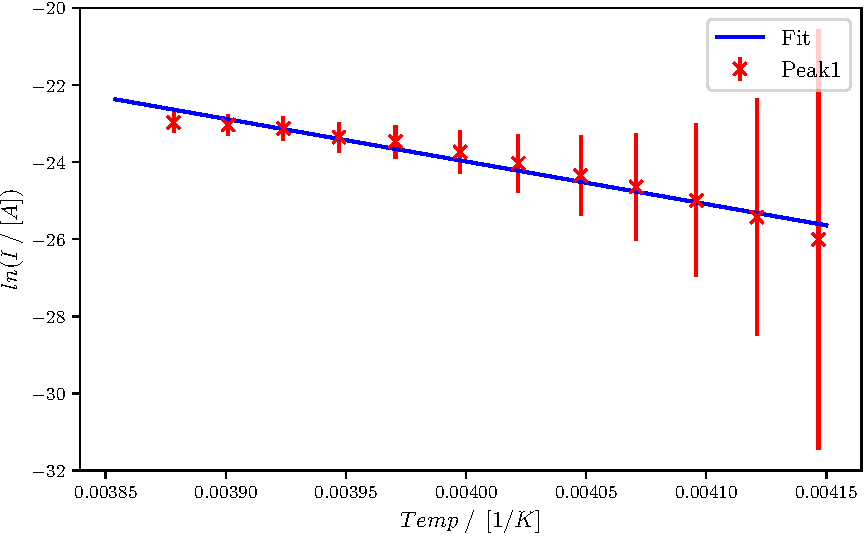
\includegraphics[width=1\textwidth]{build/2_Temp_current_peak_log_fit.pdf}
	\caption{}
	\label{fig:Auswertung_18}
\end{subfigure}%
\begin{subfigure}{.5\textwidth}
	\centering
	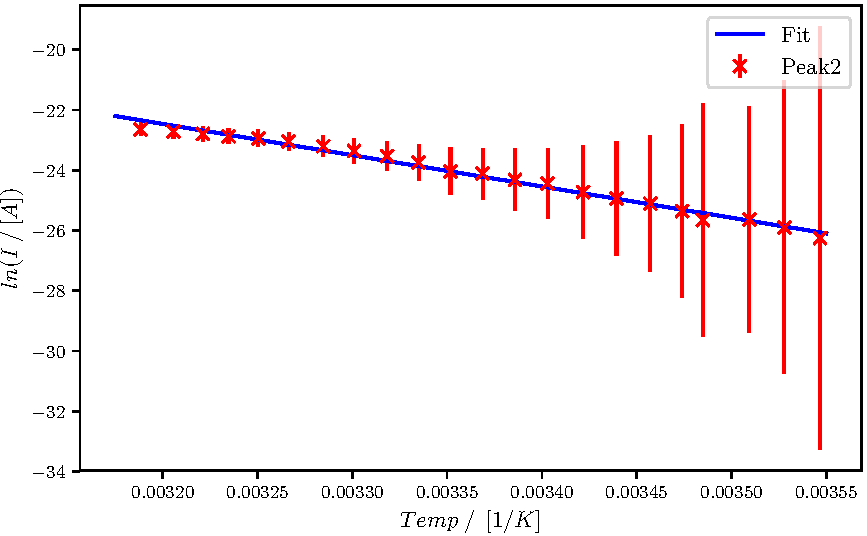
\includegraphics[width=1\textwidth]{build/2_Temp_current_peak2_log_fit.pdf}
	\caption{}
	\label{fig:Auswertung_19}
\end{subfigure}
\caption{einfach logarithmierte Darstellung der Maxima mit Ausgleichsrechnung.}
\label{fig:Auswertung_18_19}
\end{figure}

Aus den Fitparametern ergibt sich die Aktivierungsenergien $W$ zu

\begin{align}
	W_{Peak1} = \SI{0.952+-0.064}{\electronvolt}
  \quad \text{und} \quad W_{Peak2} = \SI{0.894+-0.023}{\electronvolt}
\;.
\end{align}

In die Berechnung der minimalen Relaxationszeit $\tau_0$ nach Gleichung \eqref{Formel8} geht die jeweilige Heizrate $b$ ein. Aus diesem Grund werden im Folgenden die Temperaturen im Intervall der Maxima gegen die Zeit aufgetragen (siehe Abbildung \ref{fig:Auswertung_20_21}) und es wird mit einer lineare Ausgleichsrechnung die Heizrate $b$ bestimmt. Diese ergibt sich zu:

\begin{align}
	b_{Peak1} = \SI{1.453+-0.002}{\kelvin\per\minute}
  \quad \text{und} \quad b_{Peak2} = \SI{1.477+-0.007}{\kelvin\per\minute}
\;.
\end{align}

\begin{figure}
\centering
\begin{subfigure}{.5\textwidth}
	\centering
	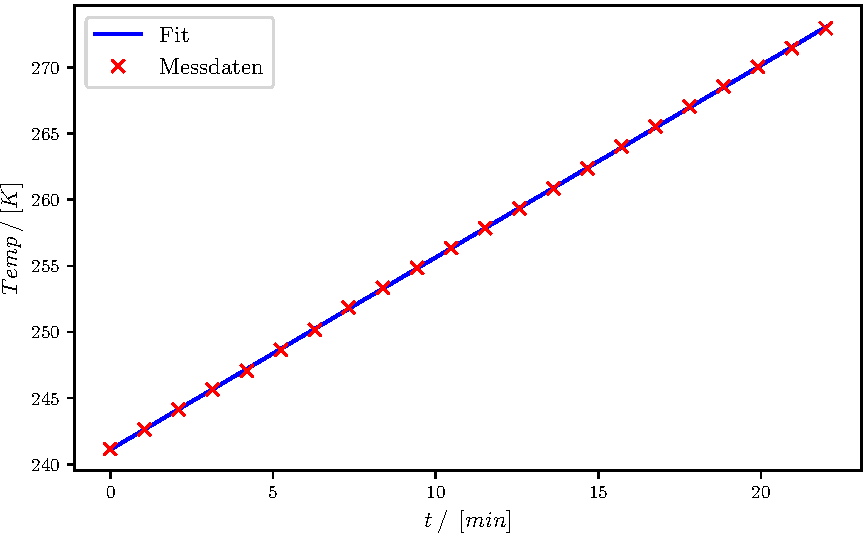
\includegraphics[width=1\textwidth]{build/2_Temp_Time_Peak1.pdf}
	\caption{}
	\label{fig:Auswertung_20}
\end{subfigure}%
\begin{subfigure}{.5\textwidth}
	\centering
	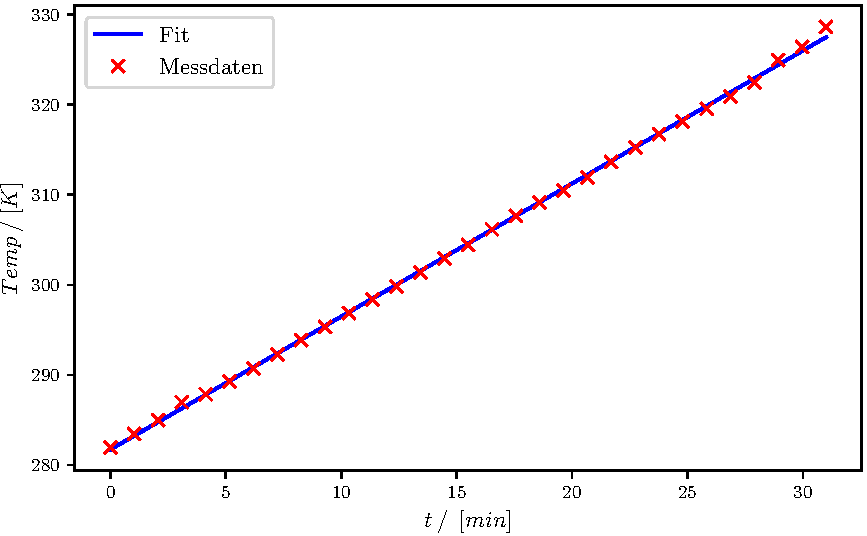
\includegraphics[width=1\textwidth]{build/2_Temp_Time_Peak2.pdf}
	\caption{}
	\label{fig:Auswertung_21}
\end{subfigure}
\caption{Darstellung der Temperatur gegen die Zeit zur Ermittlung der Heizrate während der Durchführung.}
\label{fig:Auswertung_20_21}
\end{figure}

Unter Verwendung von Gleichung \eqref{Formel5} und folgt schließlich:
\begin{align}
	T_{max,Peak1} = \SI{259.3}{\kelvin}
  \quad \text{und} \quad T_{max,Peak2} = \SI{315.2}{\kelvin}
\;.
\end{align}

ergibt sich schließlich für die minimale Relaxationszeit
\begin{align}
	\tau_{0,Peak1} = \SI{0.001+-0.004}{\pico\second}
  \quad \text{und} \quad \tau_{0,Peak2} = \SI{33+-28}{\pico\second}
\;.
\end{align}

\subsubsection{Bestimmung von $W$ mit der "Vollpeak"-Methode}

Für dieses Verfahren werden erneut die Messdaten der gesamten Maxima verwendet. Ebenfalls wird das in der Fitfunktion enthaltene Integral, wie in Gleichung \ref{eq:auswertung_integral} beschrieben, berechnet. Somit sind in Abbildung \ref{fig:Auswertung_22_23} separat die beiden Maxima mit der jeweiligen Ausgleichsrechnung (siehe Gleichung \ref{eq:auswertung_integral}) dargestellt.

\begin{figure}
\centering
\begin{subfigure}{0.5\textwidth}
	\centering
	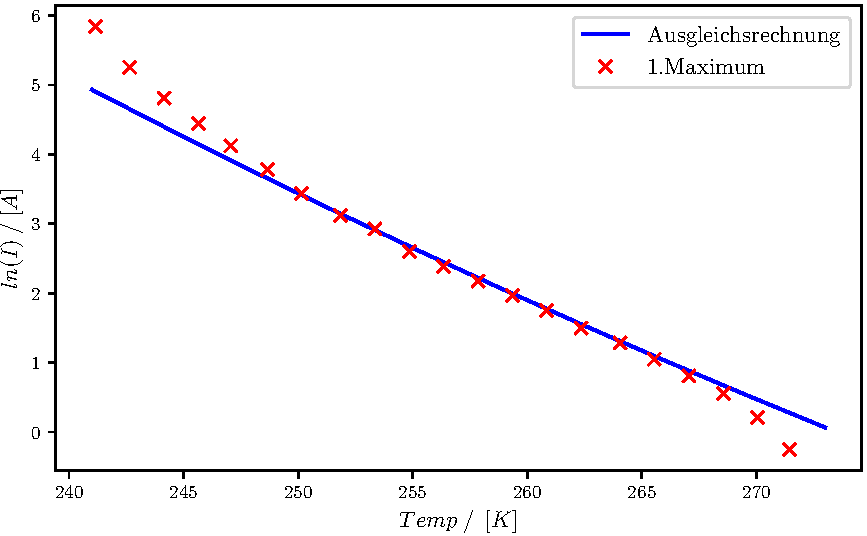
\includegraphics[width=1\textwidth]{build/2_Temp_current_peak_log_3.pdf}
	\caption{}
	\label{fig:Auswertung_22}
\end{subfigure}%
\begin{subfigure}{0.5\textwidth}
	\centering
	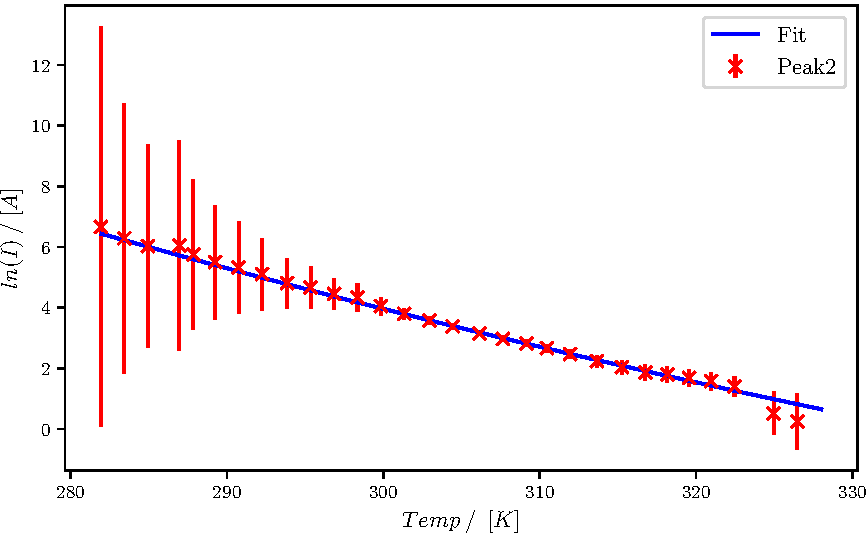
\includegraphics[width=1\textwidth]{build/2_Temp_current_peak2_log_3.pdf}
	\caption{}
	\label{fig:Auswertung_23}
\end{subfigure}
\caption{Darstellung der Messwerte mit Ausgleichsrechnung nach \ref{eq:auswertung_integral}.}
\label{fig:Auswertung_22_23}
\end{figure}


Aus den Fitparametern ergeben sich die Aktivierungsenergien 
\begin{align}
	W_{Peak1} = \SI{0.862+-0.027}{\electronvolt}
  \quad \text{und} \quad W_{Peak2} = \SI{1.002+-0.015}{\electronvolt}
\;.
\end{align}

Durch exponentieren des Fitparamters, der die Relation $\ln(\tau_0\cdot b)$ darstellt und anschließendem dividieren durch die zuvor berechnete Heizrate $b$, berechnet sich die minimale Relaxationszeit zu

\begin{align}
	\tau_{0,Peak1} = \SI{92+-113}{\atto\second}
  \quad \text{und} \quad \tau_{0,Peak2} = \SI{522+-302}{\atto\second}
\;.
\end{align}


% % Examples
% \begin{equation}latio
%   U(t) = a \sin(b t + c) + d
% \end{equation}
%
% \begin{align}
%   a &= \input{build/a.tex} \\
%   b &= \input{build/b.tex} \\
%   c &= \input{build/c.tex} \\
%   d &= \input{build/d.tex} .
% \end{align}
% Die Messdaten und das Ergebnis des Fits sind in Abbildung~\ref{fig:plot} geplottet.
%
% %Tabelle mit Messdaten
% \begin{table}
%   \centering
%   \caption{Messdaten.}
%   \label{tab:data}
%   \sisetup{parse-numbers=false}
%   \begin{tabular}{
% % format 1.3 bedeutet eine Stelle vorm Komma, 3 danach
%     S[table-format=1.3]
%     S[table-format=-1.2]
%     @{${}\pm{}$}
%     S[table-format=1.2]
%     @{\hspace*{3em}\hspace*{\tabcolsep}}
%     S[table-format=1.3]
%     S[table-format=-1.2]
%     @{${}\pm{}$}
%     S[table-format=1.2]
%   }
%     \toprule
%     {$t \:/\: \si{\milli\second}$} & \multicolumn{2}{c}{$U \:/\: \si{\kilo\volt}$\hspace*{3em}} &
%     {$t \:/\: \si{\milli\second}$} & \multicolumn{2}{c}{$U \:/\: \si{\kilo\volt}$} \\
%     \midrule
%     \input{build/table.tex}
%     \bottomrule
%   \end{tabular}
% \end{table}
%
% % Standard Plot
% \begin{figure}
%   \centering
%   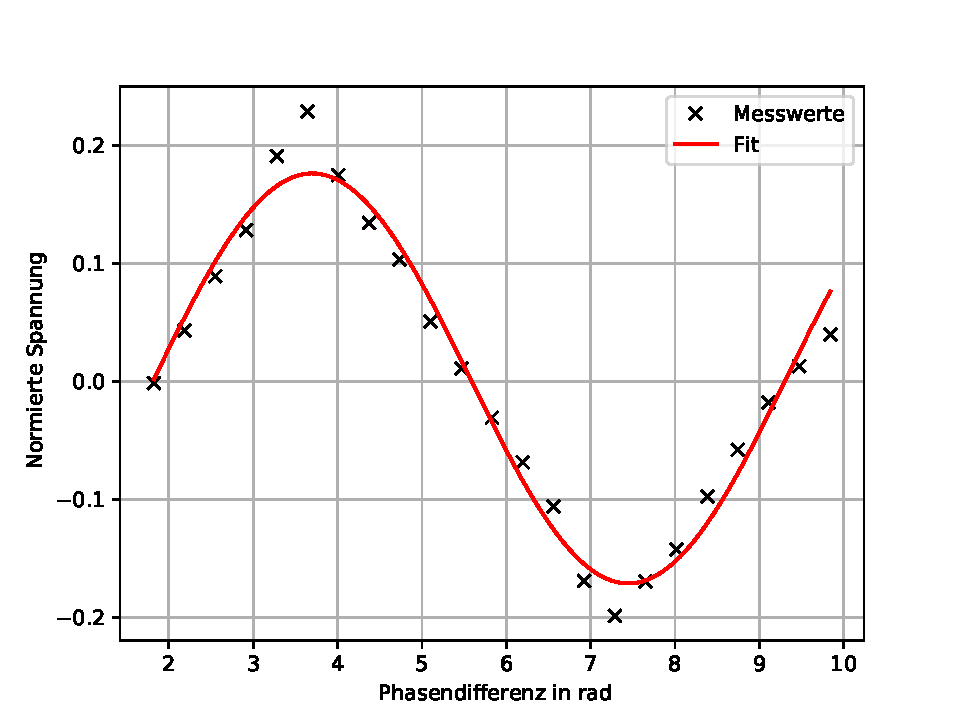
\includegraphics{build/plot.pdf}
%   \caption{Messdaten und4 Fitergebnis.}
%   \label{fig:plot}
% \end{figure}
%
% 2x2 Plot
% \begin{figure*}
%     \centering
%     \begin{subfigure}[b]{0.475\textwidth}
%         \centering
%         \includegraphics[width=\textwidth]{Abbildungen/Schaltung1.pdf}
%         \caption[]%
%         {{\small Schaltung 1.}}
%         \label{fig:Schaltung1}
%     \end{subfigure}
%     \hfill
%     \begin{subfigure}[b]{0.475\textwidth}
%         \centering
%         \includegraphics[width=\textwidth]{Abbildungen/Schaltung2.pdf}
%         \caption[]%
%         {{\small Schaltung 2.}}
%         \label{fig:Schaltung2}
%     \end{subfigure}
%     \vskip\baselineskip
%     \begin{subfigure}[b]{0.475\textwidth}
%         \centering
%         \includegraphics[width=\textwidth]{Abbildungen/Schaltung4.pdf}    % Zahlen vertauscht ... -.-
%         \caption[]%
%         {{\small Schaltung 3.}}
%         \label{fig:Schaltung3}
%     \end{subfigure}
%     \quad
%     \begin{subfigure}[b]{0.475\textwidth}
%         \centering
%         \includegraphics[width=\textwidth]{Abbildungen/Schaltung3.pdf}
%         \caption[]%
%         {{\small Schaltung 4.}}
%         \label{fig:Schaltung4}
%     \end{subfigure}
%     \caption[]
%     {Ersatzschaltbilder der verschiedenen Teilaufgaben.}
%     \label{fig:Schaltungen}
% \end{figure*}
